\chapter{Notation and Definition}

\section{Notation}

We will review all the necessary notation and mathematics for us to continue the journey of Machine Learning.

\subsection{Data Structure}

A \textbf{scalar} is simple numerical value, like $15$ or $-3.25$, denoted by an italic letter, like $x$ or $a$. A \textbf{vector} is an ordered list of scalar values, called attributes. Vector is denoted by bold character $\mathbf{x}$ or $\mathbf{w}$. A \textbf{matrix} is a rectangular array of numbers arranged in rows and columns.

\begin{figure}[H]
	\begin{subfigure}[t]{0.45\linewidth}
		\centering
		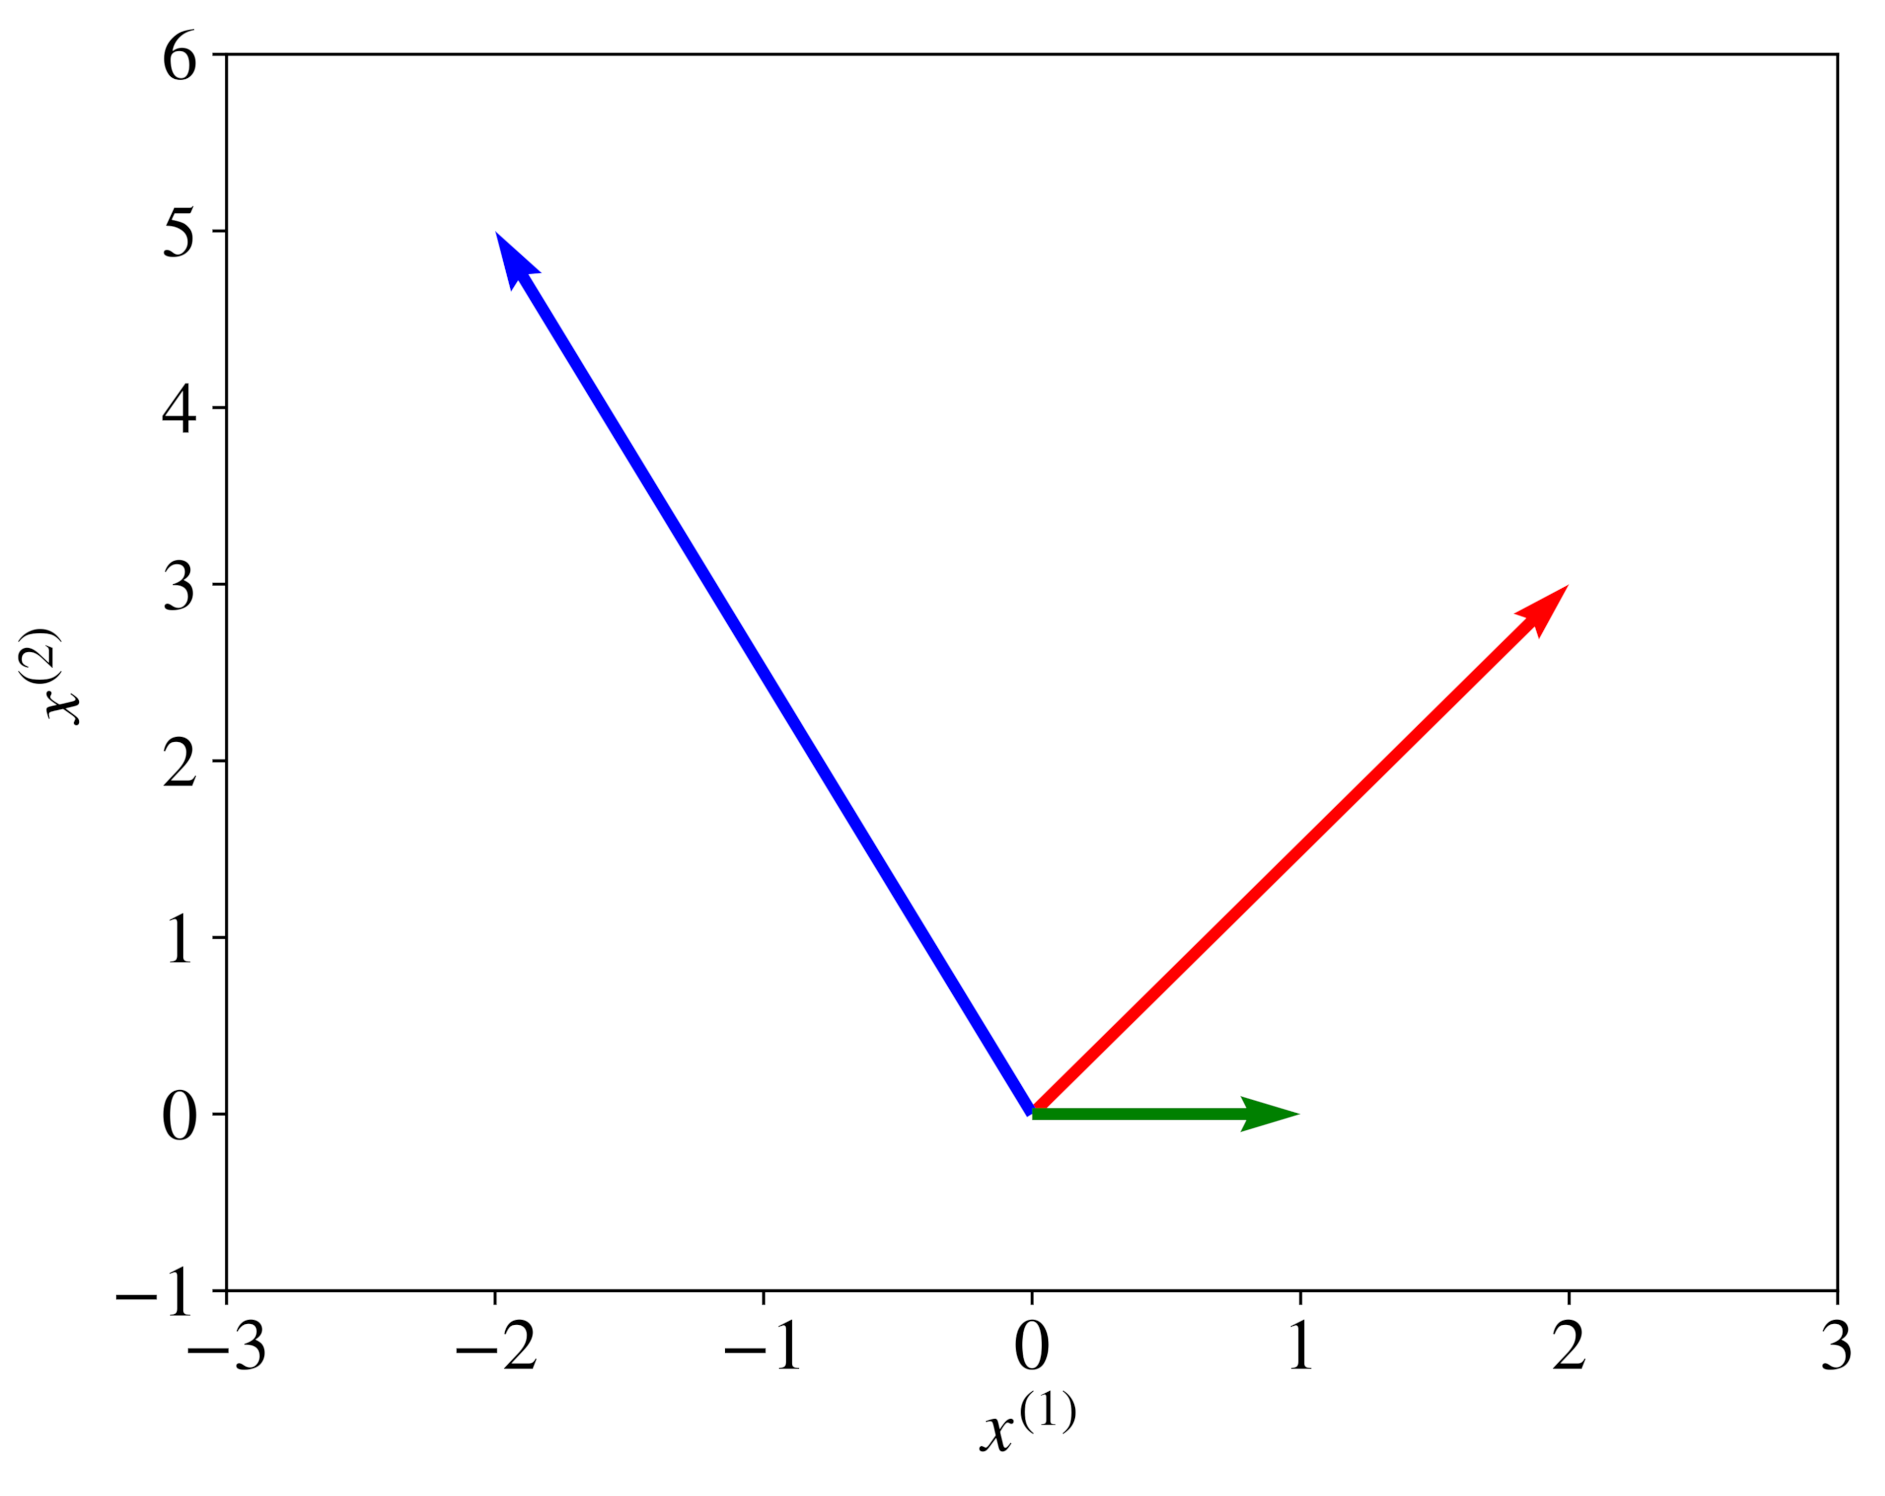
\includegraphics[width=\linewidth]{imgs/notation/notation_1}
		\caption{First subfigure}
	\end{subfigure}
	\hfill % this will put some space between your two figures
	\begin{subfigure}[t]{0.45\linewidth}
		\centering
		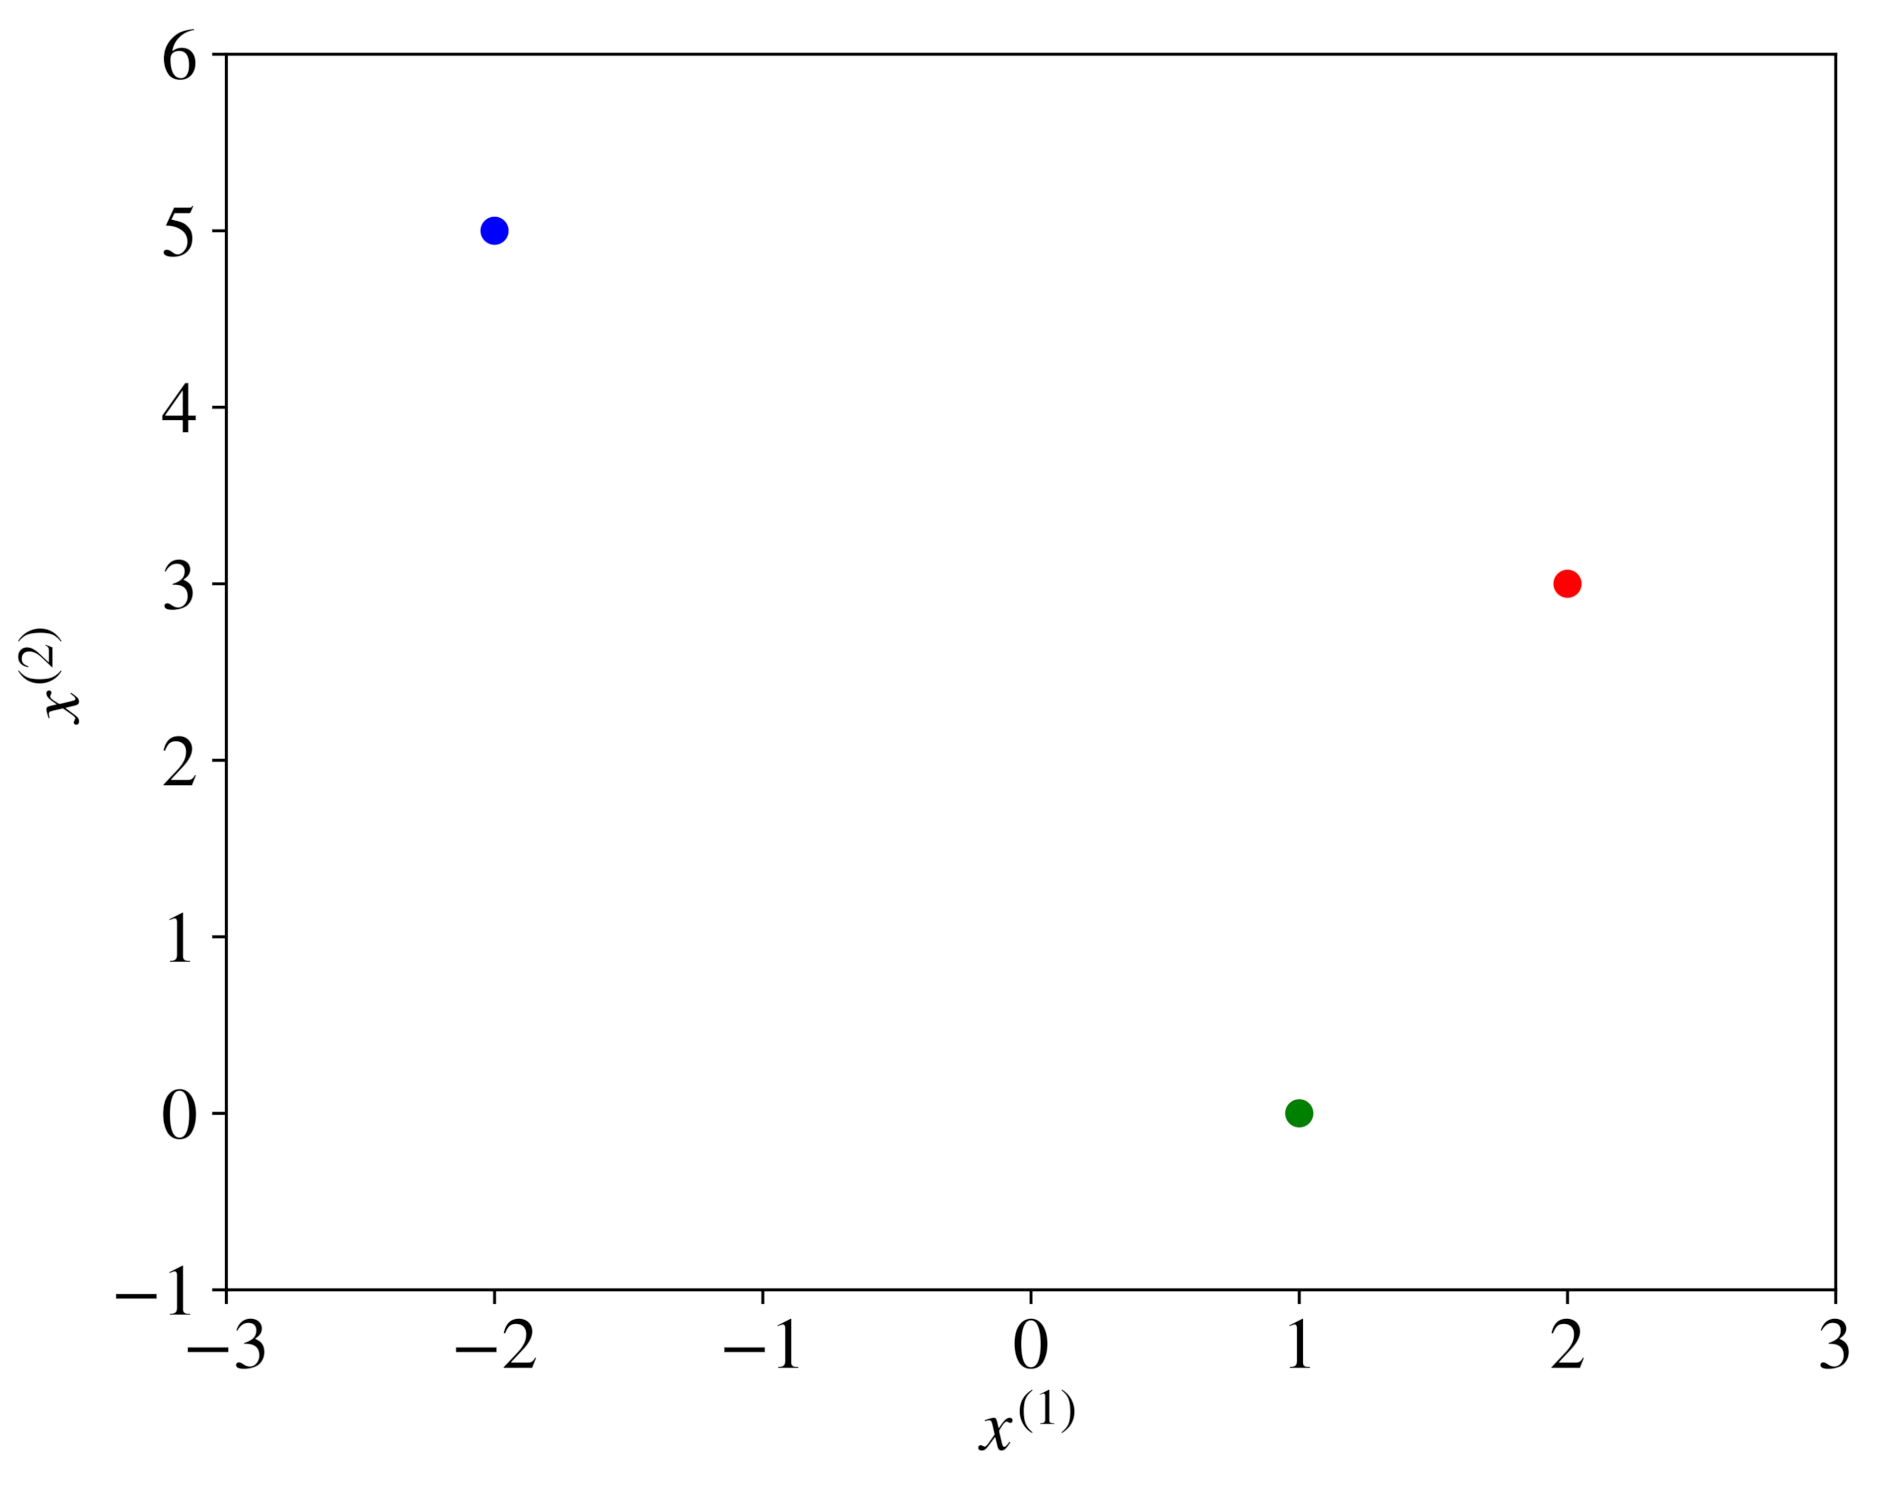
\includegraphics[width=\linewidth]{imgs/notation/notation_2}
		\caption{Second subfigure}
	\end{subfigure}
	\caption{Three vectors visualized as directions and as points.}
	\label{fig:notation_1}
\end{figure}

A \textbf{matrix} is a rectangular array of numbers arranged in rows and columns, which are denoted with bold capital letters, such as $\mathbf{A}$ or $\mathbf{W}$.  A \textbf{set} is an unordered collection of unique elements. We denote a set as a calligraphic capital character, for example, \(\mathcal{S}\). When an element belongs to a set \(\mathcal{S}\) , we write $x\in\mathcal{S}$. We can obtain a new set $\mathcal{S}_3$ as an \textbf{intersection} of two set $\mathcal{S}_1$ and $\mathcal{S}_2$, written as $\mathcal{S} \leftarrow\mathcal{S}_{1} \cap \mathcal{S}_{2}$. Also we can obtain a new set by \textbf{union}, $\mathcal{S}_3\leftarrow\mathcal{S}_1\cup\mathcal{S}_2$.

\subsection{Capital Sigma Notation}
The summation over a collection \(\mathcal{X}=\left\{x_{1}, x_{2}, \ldots, x_{n-1}, x_{n}\right\}\) or over the attributes of a vector $\mathbf{x}=\left[x^{(1)}, x^{(2)}, \ldots, x^{(m-1)}, x^{(m)}\right]$ is denoted like this:
\begin{equation*}
	\sum_{i=1}^{n} x_{i} \stackrel{\text { def }}{=} x_{1}+x_{2}+\ldots+x_{n-1}+x_{n}, \text { or else: } \sum_{j=1}^{m} x^{(j)} \stackrel{\text { def }}{=} x^{(1)}+x^{(2)}+\ldots+x^{(m-1)}+x^{(m)}
\end{equation*}
The notation $\stackrel{\text { def }}{=}$ means ``is defined as".

\subsection{Capital Pi Notation}

\begin{equation*}
	\prod_{i=1}^{n} x_{i} \stackrel{\text { def }}{=} x_{1} \cdot x_{2} \cdot \ldots \cdot x_{n-1} \cdot x_{n}
\end{equation*}
\begin{itemize}
	\item A product of elements in a collection or attributes of a vector.
\end{itemize}

\subsection{Operations on Sets}

Given the expression:
\[ \mathcal{S}^{\prime} \leftarrow \left\{x^{2} \mid x \in \mathcal{S}, x > 3\right\} \]
This notation is used to define a derived set creation operator. It means that we create a new set \( \mathcal{S}^{\prime} \) by including the square of each element \( x \) from the set \( \mathcal{S} \), under the condition that \( x \) is greater than 3. In other words, \( \mathcal{S}^{\prime} \) is comprised of the squares of all elements in \( \mathcal{S} \) which are greater than 3.

Additionally, the cardinality operator \( |\mathcal{S}| \) is used to denote the number of elements in the set \( \mathcal{S} \). For example, if \( \mathcal{S} = \{1, 2, 4, 5\} \), then \( \mathcal{S}^{\prime} = \{16, 25\} \) as only 4 and 5 from \( \mathcal{S} \) satisfy the condition \( x > 3 \). The \textbf{cardinality} \( |\mathcal{S}| \) in this case would be 4.

\subsection{Operations on Vectors}

\textbf{Vector Addition and Subtraction:}
The sum and difference of two vectors \( \mathbf{x} \) and \( \mathbf{z} \) are defined component-wise as:
\[ \mathbf{x} + \mathbf{z} = \left[x^{(1)} + z^{(1)}, \ldots, x^{(m)} + z^{(m)}\right] \]
\[ \mathbf{x} - \mathbf{z} = \left[x^{(1)} - z^{(1)}, \ldots, x^{(m)} - z^{(m)}\right] \]
\emph{Example:} For \( \mathbf{x} = [1, 2] \) and \( \mathbf{z} = [3, 4] \),
\[ \mathbf{x} + \mathbf{z} = [1+3, 2+4] = [4, 6] \]

\textbf{Scalar Multiplication:}
A vector multiplied by a scalar \( c \) results in a scaled vector:
\[ \mathbf{x} c = \left[c x^{(1)}, \ldots, c x^{(m)}\right] \]
\emph{Example:} For \( \mathbf{x} = [1, 2] \) and \( c = 3 \),
\[ \mathbf{x} c = [3 \times 1, 3 \times 2] = [3, 6] \]

\textbf{Dot Product:}
The dot product of two vectors \( \mathbf{w} \) and \( \mathbf{x} \) is a scalar:
\[ \mathbf{w} \mathbf{x} = \sum_{i=1}^{m} w^{(i)} x^{(i)} \]
\emph{Example:} For \( \mathbf{w} = [1, 2] \) and \( \mathbf{x} = [3, 4] \),
\[ \mathbf{w} \mathbf{x} = 1 \times 3 + 2 \times 4 = 3 + 8 = 11 \]
\textbf{Matrix-Vector Multiplication:}
Multiplying a matrix \( \mathbf{W} \) by a vector \( \mathbf{x} \) yields another vector. For example:
$$
	\begin{aligned}
		\mathbf{W} \mathbf{x} & =\left[\begin{array}{lll}
				                               w^{(1,1)} & w^{(1,2)} & w^{(1,3)} \\
				                               w^{(2,1)} & w^{(2,2)} & w^{(2,3)}
			                               \end{array}\right]\left[\begin{array}{l}
				                                                       x^{(1)} \\
				                                                       x^{(2)} \\
				                                                       x^{(3)}
			                                                       \end{array}\right]                                      \\
		                      & \stackrel{\text { def }}{=}\left[\begin{array}{l}
				                                                         w^{(1,1)} x^{(1)}+w^{(1,2)} x^{(2)}+w^{(1,3)} x^{(3)} \\
				                                                         w^{(2,1)} x^{(1)}+w^{(2,2)} x^{(2)}+w^{(2,3)} x^{(3)}
			                                                         \end{array}\right] \\
		                      & =\left[\begin{array}{l}
				                               \mathbf{w}^{(1)} \mathbf{x} \\
				                               \mathbf{w}^{(2)} \mathbf{x}
			                               \end{array}\right]
	\end{aligned}
$$

\emph{Example:} For
\[ \mathbf{W} = \left[\begin{array}{ll}
			1 & 2 \\
			3 & 4
		\end{array}\right] \text{ and } \mathbf{x} = \left[\begin{array}{l}
			5 \\
			6
		\end{array}\right], \]
\[ \mathbf{W} \mathbf{x} = \left[\begin{array}{l}
			1 \times 5 + 2 \times 6 \\
			3 \times 5 + 4 \times 6
		\end{array}\right] = \left[\begin{array}{l}
			17 \\
			39
		\end{array}\right] \]
\textbf{Transpose and Multiplication:}
For the transpose of a vector \( \mathbf{x} \) denoted \( \mathbf{x}^{\top} \), and a matrix \( \mathbf{W} \), the multiplication \( \mathbf{x}^{\top} \mathbf{W} \) is given by:
$$
	\begin{aligned}
		\mathbf{x}^{\top} \mathbf{W} & =\left[\begin{array}{ll}
				                                      x^{(1)} & x^{(2)}
			                                      \end{array}\right]\left[\begin{array}{lll}
				                                                              w^{(1,1)} & w^{(1,2)} & w^{(1,3)} \\
				                                                              w^{(2,1)} & w^{(2,2)} & w^{(2,3)}
			                                                              \end{array}\right]                                                                                      \\
		                             & \stackrel{\text { def }}{=}\left[w^{(1,1)} x^{(1)}+w^{(2,1)} x^{(2)}, w^{(1,2)} x^{(1)}+w^{(2,2)} x^{(2)}, w^{(1,3)} x^{(1)}+w^{(2,3)} x^{(2)}\right]
	\end{aligned}
$$

\emph{Example:} For
\[ \mathbf{x} = \left[\begin{array}{l}
			7 \\
			8
		\end{array}\right] \text{ and } \mathbf{W} = \left[\begin{array}{lll}
			1 & 2 & 3 \\
			4 & 5 & 6
		\end{array}\right], \]
\[ \mathbf{x}^{\top} \mathbf{W} = \left[\begin{array}{lll}
			7 \times 1 + 8 \times 4, 7 \times 2 + 8 \times 5, 7 \times 3 + 8 \times 6
		\end{array}\right] = \left[\begin{array}{lll}
			39, 54, 69
		\end{array}\right] \]

\subsection{Functions}

\textbf{Definition of a Function}\\
A function is a relation that associates each element \( x \) of a set \( \mathcal{X} \), known as the domain, to a single element \( y \) of another set \( \mathcal{Y} \), known as the codomain. This relation is denoted as \( y = f(x) \), where \( f \) is the name of the function, \( x \) is the input or argument, and \( y \) is the output. The input variable is also referred to as the variable of the function.

\emph{Example:} Consider the function \( f(x) = x^2 \) defined on the domain \( \mathcal{X} = \mathbb{R} \). For \( x = 2 \), the output is \( f(2) = 2^2 = 4 \).

\textbf{Local and Global Minima}\\
The function \( f(x) \) has a local minimum at \( x = c \) if \( f(x) \geq f(c) \) for every \( x \) in an open interval around \( c \). An open interval, such as \( (0,1) \), includes all numbers between its endpoints but not the endpoints themselves. The smallest value among all local minima is known as the global minimum.

\emph{Example:} In the function \( f(x) = (x-1)^2 \), the local (and global) minimum occurs at \( x = 1 \) since \( f(x) \geq f(1) = 0 \) for all \( x \).

\begin{figure}[H]
	\centering
	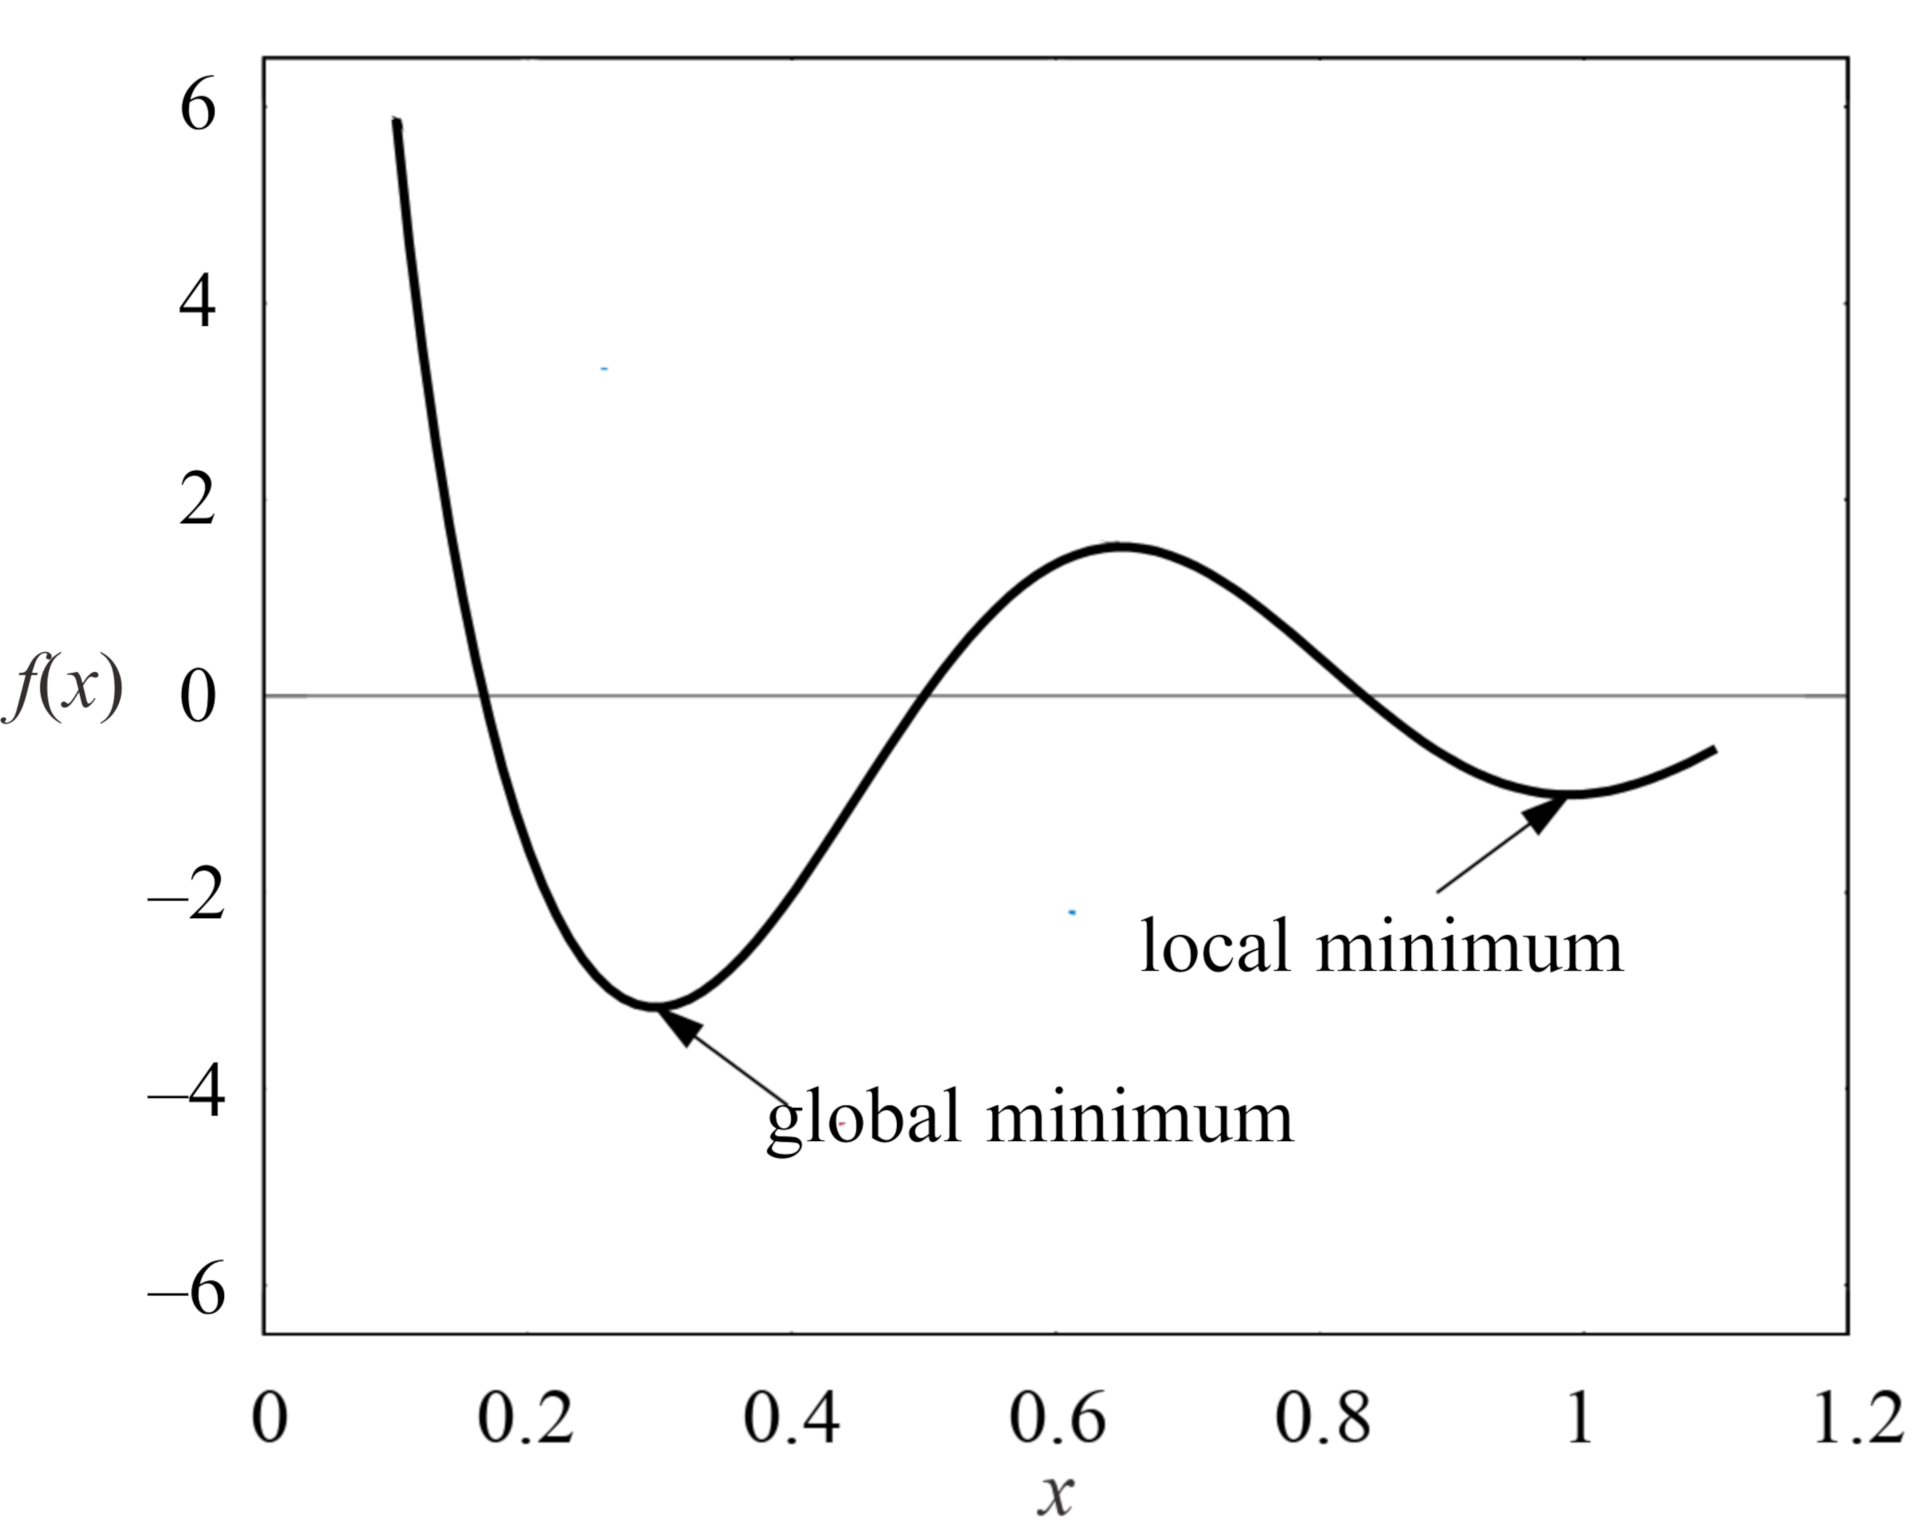
\includegraphics[width=0.7\linewidth]{imgs/notation/notation_3.png}
	\caption{A local and a global minima of a function.}
	\label{fig:notation_3}
\end{figure}

\textbf{Vector Functions}\\
A vector function, denoted \( \mathbf{y} = \mathbf{f}(x) \), is a function that returns a vector \( \mathbf{y} \). Its argument can be either a vector or a scalar.

\emph{Example:} For the vector function \( \mathbf{f}(x) = [x, x^2] \), with \( x = 2 \), the output is \( \mathbf{f}(2) = [2, 2^2] = [2, 4] \).

\subsection{Max and Arg Max}

Given a set of values \( \mathcal{A} = \{a_{1}, a_{2}, \ldots, a_{n}\} \), the operator \( \max_{a \in \mathcal{A}} f(a) \) returns the highest value of \( f(a) \) for all elements in the set \( \mathcal{A} \). Conversely, the operator \( \arg \max_{a \in \mathcal{A}} f(a) \) identifies the specific element \( a \) in the set \( \mathcal{A} \) that maximizes the function \( f(a) \).

In cases where the set is implicit or infinite, we can use the notation \( \max_{a} f(a) \) or \( \arg \max_{a} f(a) \) respectively. Similarly, the operators \( \min \) and \( \arg \min \) function in a comparable way, determining the lowest value of a function and the

\subsection{Assignment Operator}
The expression \(a \leftarrow f(x)\) means that the variable \(a\) gets the new value: the result of \(f(x)\). We say that the variable \(a\) gets assigned a new value. Similarly, \(\mathbf{a} \leftarrow\left[a_{1}, a_{2}\right]\) means that the vector variable \(\mathbf{a}\) gets the two-dimensional vector \(\left[a_{1}, a_{2}\right]\).

\subsection{Derivative and Gradient}
A \textbf{derivative} \(f^{\prime}\) of a function \(f\) is a function or a value that describes how fast \(f\) grows (or decreases). If the derivative \(f^{\prime}\) is a function, then the function \(f\) can grow at a different pace in different regions of its domain.

we can use \textbf{chain rule} when we encounter hard-to-differentiate function. For instance if \(F(x)=f(g(x))\), where \(f\) and \(g\) are some functions, then \(F^{\prime}(x)= f^{\prime}(g(x)) g^{\prime}(x)\).

\textbf{Gradient} is the generalization of derivative for functions that take several inputs (or one input in the form of a vector or some other complex structure). A gradient of a function is a vector of \textbf{partial derivatives}. For example, \(f\left(\left[x^{(1)}, x^{(2)}\right]\right)=a x^{(1)}+b x^{(2)}+c\), then the partial derivative of function \(f\) \textit{with respect to} \(x^{(1)}\), denoted as \(\frac{\partial f}{\partial x^{(1)}}\), is given by,